
We use a $K$-correction based on the BC03 stellar population spectral
models to convert the observed $z_{850}$ magnitude to a rest-frame $B$
magnitude for each cluster. The BC03 models consist of galaxy spectra
for an instantaneous starburst (``simple stellar population'', or SSP)
with various initial metallicities ($0.0001 < Z < 0.1$) and ages
($1 \times 10^5$ -- $2 \times 10^{10}$ yr). BC03 contains models for
several different stellar evolution prescriptions, and two initial
mass functions (IMF). We use the recommended Padova 1994 stellar
evolution prescription and Chabrier IMF. Figure~\ref{fig:bc03spectra}
shows examples of BC03 spectra for metallicity $Z=0.02$ at a range of
ages. Also shown are the rest-frame $U$ and $B$ bands, as well as the
observed $i_{775}$ and $z_{850}$ bands at the minimum ($0.91$) and
maximum ($1.50$) redshift of clusters in the sample. The $z_{850}$
filter is a good match to rest-frame $B$ band across much of the
redshift range of the clusters. It is the best match at $z \approx
1.07$ and shifts progressively bluer than $B$ at higher redshifts,
approximately matching $U$ at the high-redshift end of the sample.

\begin{figure}[t]
\begin{center}
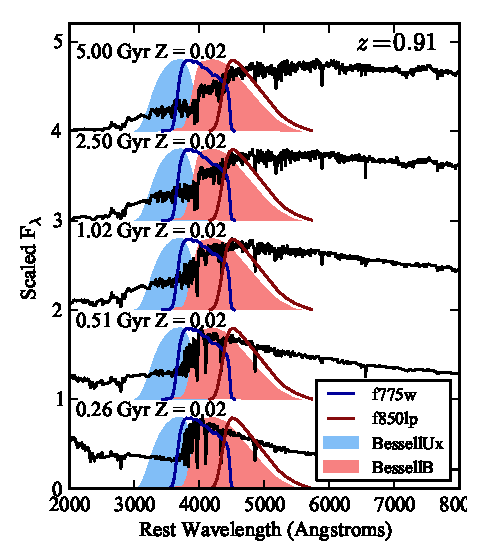
\includegraphics{figures/clrate/bc03spectra_lowz.eps}%
\includegraphics{figures/clrate/bc03spectra_highz.eps}
\end{center}
\caption[Examples of Bruzual \& Charlot (2003) spectra]{Examples
of BC03 spectra for a single initial metallicity ($Z =
0.02$) and a range of ages. The left and right panels are identical,
except that the \emph{left panel} shows the observed filters at $z=0.91$ and
the \emph{right panel} shows them at $z=1.50$ (the approximate range
of cluster redshifts).\label{fig:bc03spectra}}
\end{figure}

Rather than using a single $K$-correction for all the light in each
cluster, we apply a $K$-correction to each galaxy magnitude based on
its $i_{775}-z_{850}$ color. For each cluster's redshift, we determine
the relation between $K$-correction ($M_B$ (rest) $- z_{850}$) and
$i_{775}-z_{850}$ color, using BC03 spectra with initial metallicities
in the range $0.004 < Z < 0.05$ and ages in the range $1 \times 10^8 -
5 \times 10^9$~yr. This relation is shown for four example cluster
redshifts in Figure~\ref{fig:kcorr} (left panels). The colored lines
in each panel represent BC03 spectra with constant metallicity and age
increasing from $1 \times 10^8$ -- $5 \times 10^9$ yr.  For most
cluster redshifts in our sample, all of the spectra over this wide
range fall along the same line in $K$-correction versus color, meaning
that the color determines the $K$-correction, regardless of the
metallicity or age assumed. At $z=1.07$, where the best match between
$z_{850}$ and rest-frame $B$ is obtained, the $K$-correction is nearly
independent of color or model, as one would expect. In the redshift
range $1.15 \lesssim z \lesssim 1.4$, the curves are multi-valued for
a range of observed colors, and are the most dispersed at $z \approx
1.26$ (shown in Figure~\ref{fig:kcorr}). To select a $K$-correction
given an observed galaxy color, we average the $K$-correction for all
models with similar colors, arriving at the black line shown in each
panel.

\begin{figure}[p]
\begin{center}
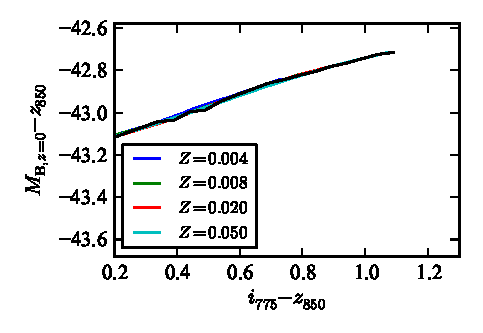
\includegraphics[width=0.45\textwidth]{figures/clrate/kcorr_mag_z1.eps}%
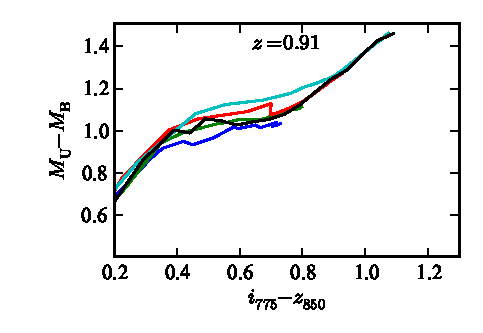
\includegraphics[width=0.45\textwidth]{figures/clrate/kcorr_color_z1.eps}
\includegraphics[width=0.45\textwidth]{figures/clrate/kcorr_mag_z2.eps}%
\includegraphics[width=0.45\textwidth]{figures/clrate/kcorr_color_z2.eps}
\includegraphics[width=0.45\textwidth]{figures/clrate/kcorr_mag_z3.eps}%
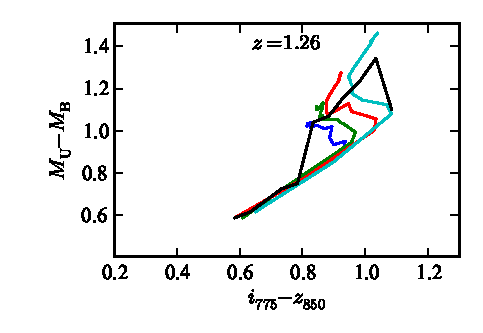
\includegraphics[width=0.45\textwidth]{figures/clrate/kcorr_color_z3.eps}
\includegraphics[width=0.45\textwidth]{figures/clrate/kcorr_mag_z4.eps}%
\includegraphics[width=0.45\textwidth]{figures/clrate/kcorr_color_z4.eps}
\end{center}
\caption[$K$-correction fits to Bruzual \& Charlot (2003)
spectra]{$K$-correction fits, based on BC03 spectra.  The colored
lines in each panel represent BC03 spectra with constant initial
metallicity and age increasing from $1 \times 10^8$ -- $5 \times 10^9$
yr. The black line is the relation used in this analysis. The \emph{left
panels} show the $K$-correction as a function of observed galaxy color
and the \emph{right panels} show the rest-frame $U-B$ color as a function of
observed color. \label{fig:kcorr}}
\end{figure}

The dispersion of the models about the best-fit line is $<0.03$~mag at
redshifts $\lesssim 1.1$ and $\gtrsim 1.4$, and reaches its largest
value of 0.09~mag at $z=1.26$. We calculate the $K$-correction for
each galaxy using this best-fit relation, effectively assuming that
every galaxy is at the cluster redshift. This results in an incorrect
luminosity for non-cluster member galaxies, but this is accounted for
by performing the same $K$-correction on the galaxies in the GOODS
fields prior to subtracting their luminosity. 


\vspace{1.2in}


% From draft:

%For all remaining galaxies, I convert the observed $z_{850}$
%magnitude into an absolute rest-frame $B$ magnitude, {\it assuming}
%the galaxy is at the cluster redshift. (Of course, this will not give
%an accurate $B$ magnitude for galaxies not in the cluster, but
%following the same procedure for the ``background'' fields will mean
%that the correct magnitude is subtracted.) To make this
%$K$-correction, I use the stellar population synthesis models
%of BC03.


%In computing the $K$-correction for each cluster, I consider spectra
%with initial metallicity 0.004, 0.008, 0.02, and 0.05, and in the age
%range $1 \times 10^8$ -- $5 \times 10^9$ yr. For each spectrum in this
%range, I compute the $i_{775} - z_{850}$ color (with the spectrum
%redshifted to the cluster redshift), the $U - B$ rest-frame color, and
%$M_{B,z=0}-z_{850}$, which is the difference between the observed
%$z_{850}$ magnitude and the absolute rest-frame $B$ magnitude
%(assuming the spectrum is at the cluster redshift). Plotting
%$M_{B,z=0}-z_{850}$ against $i_{775} - z_{850}$ gives the
%$K$-correction as a function of the observed galaxy color.


%This line is used to convert the
%observed $z_{850}$ magnitude to a rest-frame absolute $B$ magnitude
%for each galaxy, given its color. The standard deviation of the
%residuals of the models from this best fit line are 0.004, 0.004,
%0.094, and 0.024 magnitudes, for redshifts 0.91, 1.07, 1.26 and 1.45,
%respectively. Thus, for most clusters, we expect the error associated
%with the $K$-correction to be quite negligible (less than 3\%), and
%even in the worst cases, should generally be below 10\%. For galaxies
%with colors outside the range of models, the model with the nearest
%color is used to $K$-correct, in order to avoid errors from
%extrapolating the fit far beyond the fitted range. Because galaxies
%with these extreme colors are most likely not part of the cluster, any
%errors will cancel out when the background is subtracted. In the right
%panels of Figure~\ref{fig:kcorr} the rest-frame $U-B$ color is shown
%as a function of observed color, exhibiting similar
%characteristics. The standard deviation of residuals for color are
%0.030, 0.010, 0.106, and 0.025 magnitudes, for redshifts 0.91, 1.07,
%1.26 and 1.45, respectively.
